\section{Komplexe Zahlen $\mathbb{C}$}
Eine komplexen Zahl $z$ ist ein geordnetes Paar $(x; y)$ aus zwei reellen Zahlen $x$ und $y$: $z = x + \mathrm j y$.
$x$ ist der Realteil von $z$, $y$ heisst Imaginärteil von $z$. Die imaginäre Einheit heisst $j$. Es gilt:
\begin{equation*}
	\mathrm j^2 = -1
\end{equation*}

\subsection{Darstellungsformen}
\settowidth{\MyLenA}{Trigonometrische Form~~}
\begin{tabular}{@{}p{\the\MyLenA}%
				@{}p{\linewidth - \the\MyLenA}}
Normalform & $z = x + \mathrm j y$ \\
Trigonometrische Form & $z = r \cdot (\cos \varphi + \mathrm j \sin \varphi)$\\
Exponentialform & $z = r \cdot \mathrm e^{\mathrm j \varphi}$
\end{tabular}

\begin{center}
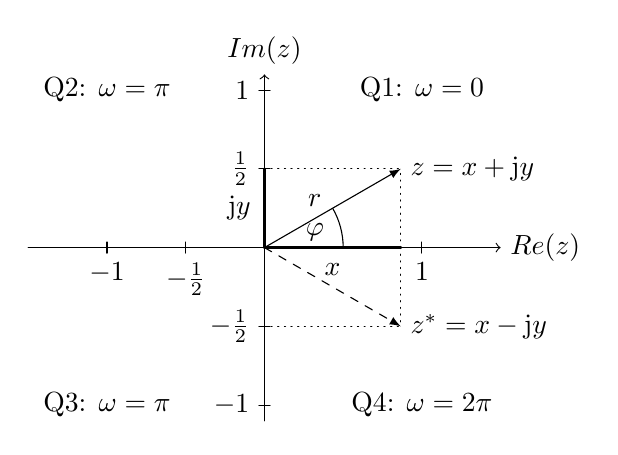
\begin{tikzpicture}[scale=2,cap=round]
  \def\costhirty{0.8660256}
  \def\sinthirty{0.5}
  % Colors
  \colorlet{lightgrey}{white!80!black}

  % Styles
  \tikzstyle{axes}=[]
  \tikzstyle{important line}=[very thick]
  \tikzstyle{vector}=[-latex]

  % The graphic
  \draw[style=help lines,step=0.5cm] (-1.1,-1.1);

  \begin{scope}[style=axes]
    \draw[->] (-1.5,0) -- (1.5,0) node[right] {$Re(z)$};
    \draw[->] (0,-1.1) -- (0,1.1) node[above] {$Im(z)$};

    \foreach \x/\xtext in {-1, -.5/-\frac{1}{2}, 1}
      \draw[xshift=\x cm] (0pt,1pt) -- (0pt,-1pt) node[below,fill=white]
            {$\xtext$};

    \foreach \y/\ytext in {-1, -.5/-\frac{1}{2}, .5/\frac{1}{2}, 1}
      \draw[yshift=\y cm] (1pt,0pt) -- (-1pt,0pt) node[left,fill=white]
            {$\ytext$};
  \end{scope}

  \draw[style=important line]
    (0,0) -- node[left=1pt,fill=white] {$\mathrm j y$} +(0,\sinthirty);

  \draw[style=important line]
    (0,0) -- node[below=2pt,fill=white] {$x$} (\costhirty,0);

  \draw[vector] (0,0) -- (\costhirty, \sinthirty) node [right,fill=white] {$z = x + \mathrm j y$};

  \draw[dotted] (0,\sinthirty) -- (\costhirty, \sinthirty);

  \draw[dotted] (\costhirty,0) -- (\costhirty, \sinthirty);

  \draw[dotted] (\costhirty,0) -- (\costhirty, -\sinthirty);

  \draw[dotted] (0,-\sinthirty) -- (\costhirty, -\sinthirty);

  \draw[vector, dashed] (0,0) -- (\costhirty, -\sinthirty) node [right,fill=white] {$z^* = x - \mathrm j y$};

  \node (q1) at (1,1) {Q1: $\omega = 0$};
  \node (q2) at (-1, 1) {Q2: $\omega = \pi$};
  \node (q3) at (-1, -1) {Q3: $\omega = \pi$};
  \node (q4) at (1, -1) {Q4: $\omega = 2\pi$};
  \node (z) at (0.32, 0.3) {$r$};
  \node (phi) at (0.32, 0.1) {$\varphi$};
  \draw (0.5,0) arc (0:30:5mm);
\end{tikzpicture}
\end{center}

\subsection{Umrechnungen}
\subsubsection{Trigonometrisch/Exponential Form $\rightarrow$ Normalform}
\begin{align*}
	x& = r \cdot \cos \varphi\\
	y& = r \cdot \sin \varphi
\end{align*}

\subsubsection{Normalform $\rightarrow$ Trigonometrisch/Exponentialform}
\begin{align*}
	r = |z|& = \sqrt{x^2 + y^2}\\
	\varphi& = \arctan \left(\frac{y}{x}\right) + \omega
\end{align*}
Dabei heissen $r$ der Betrag und $\varphi$ Argument/Winkel/Phase von $z$.\\
$\omega$ ist abhängig vom Quadranten.

\subsection{Anmerkungen}
\begin{itemize}\itemsep0em
	\item $\mathbb{C} = \{z | z = x + \mathrm j y$ mit $x, y \in \mathbb{R}\}$
	\item $z_1 = x_1 + \mathrm j y_1  = z_2 = x_2 + \mathrm j y_2 \Rightarrow (x_1 = x_2) \wedge (y_1 = y_2)$
	\item Die konjugiert komplexe Zahl $z^* = (x + \mathrm j y)^* = x - \mathrm j y$.
	\item $e^{\mathrm j \pi} = -1$
\end{itemize}
